\subsection*{Actividad 1.3}

Modelos de automóvil 1 y 2.

\begin{align*}
    D_1 &= t &
    D_2 &= \frac{t^2}{2}
\end{align*}

\subsubsection*{Parte A}

\textbf{a)} Representación gráfica de los dos modelos.

\begin{center}
\begin{tikzpicture}
\begin{axis}[
    axis lines = left,
    xlabel = \(t\),
    ylabel = {\(D(t)\)},
    clip = false,
]
% D_1
\addplot [
    domain=0:10, 
    samples=200, 
    color=blue,
]
{x};
\addlegendentry{\(D_1=t\)}

% D_2
\addplot[
    domain=0:10,
    samples=200,
    color=red,
]
{x*x/2};
\addlegendentry{\(D_2=\frac{t^2}{2}\)}
\end{axis}
\end{tikzpicture}
\end{center}

\textbf{b)} Kilómetros recorridos al cabo de 1, 2 y 3 minutos.

\begin{center}
\begin{tabular}{ c c c }
	t	&	$D_1$  &   $D_2$  \\
	\hline \\
	1	&	1     &   $1/2$\\	
	2	&	2     &   2\\	
	3	&	3     &   $9/2$\\
    \hline
\end{tabular}
\end{center}

\textbf{c)} Velocidad media en intervalos [0, 1], [0, 2], [0, 3] y [1, 2].

\begin{center}
\begin{tabular}{ c c c }
	Intervalo	&	$D_1$  &   $D_2$ \\
	\hline \\
	$[0, 1]$    &	 1     &   $1/2$ \\	
	$[0, 2]$    &	 1     &   1     \\	
	$[0, 3]$    &	 1     &   $3/2$ \\
    $[1, 2]$    &    1     &   $3/2$ \\
    \hline
\end{tabular}
\end{center}

\textbf{Conclusiones.} Si observamos la velocidad media del modelo 1, rápidamente notamos que esta es constante a lo largo de la trayectoria. Esto es lo esperable de un modelo lineal. Al ser constante la pendiente, es esperable que el cambio en la misma, cualquiera sea el punto que se tome, permanezca constante, como se ha observado en el modelo anterior.

En lo que respecta al modelo 2, la situación es diferente. Nos encontramos ahora frente a un modelo cuadrático, por lo cual el cálculo de la velocidad media cambia según el período de tiempo considerado, siendo superior a medida que pasa el tiempo. 

Ello llevaría a concluir que uno de los automóviles se desplaza de manera uniforme, mientras el otro lo hace de manera uniformemente variada.

\vspace{10pt}

\textbf{d)} Para calcular la velocidad en los minutos 1 y 2 recurrimos a la derivada de cada una de las funciones:

\begin{align*}
    D_1' &= 1 &
    D_2' &= t
\end{align*}

\begin{center}
\begin{tabular}{ c c c }
	t	&	$D'_1$  &   $D'_2$  \\
	\hline \\
	1	&	1     &   1\\	
	2	&	1     &   2\\
    \hline
\end{tabular}
\end{center}

\textbf{e)} Las tangentes a la distancia recorrida por el automóvil 2, en los puntos 1 y 2, son las siguientes:

\begin{center}
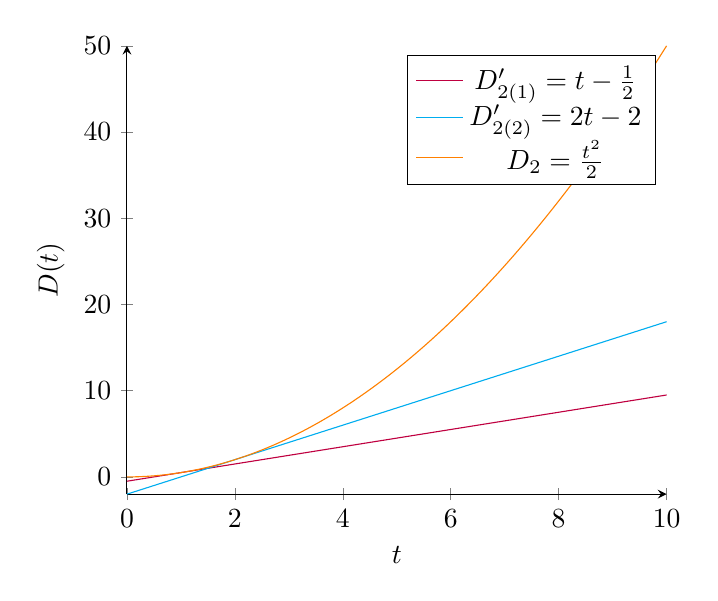
\begin{tikzpicture}
\begin{axis}[
    axis lines = left,
    xlabel = \(t\),
    ylabel = {\(D(t)\)},
    clip = false,
]
% D'_2 en 1
\addplot [
    domain=0:10, 
    samples=200, 
    color=purple,
]
{x-0.5};
\addlegendentry{\(D'_{2(1)}=t-\frac{1}{2}\)}

% D'_2 en 1
\addplot [
    domain=0:10, 
    samples=200, 
    color=cyan,
]
{2*x-2};
\addlegendentry{\(D'_{2(2)}=2t-2\)}

% D_2
\addplot[
    domain=0:10,
    samples=200,
    color=orange,
]
{x*x/2};
\addlegendentry{\(D_2=\frac{t^2}{2}\)}
\end{axis}
\end{tikzpicture}
\end{center}

Las expresiones de las rectas tangentes se obtienen recurriendo a la notación punto-pendiente ($y-y_0 = m(x-x_0)$), despejando la $y$.

\vspace{10pt}

\textbf{f)} Como se desprende tanto de la tabla como de la representación gráfica, la velocidad del automóvil 1 es constante, mientras la del automóvil 2 se incrementa a medida que pasa el tiempo.
